% Options for packages loaded elsewhere
\PassOptionsToPackage{unicode}{hyperref}
\PassOptionsToPackage{hyphens}{url}
%
\documentclass[
]{article}
\usepackage{amsmath,amssymb}
\usepackage{iftex}
\ifPDFTeX
  \usepackage[T1]{fontenc}
  \usepackage[utf8]{inputenc}
  \usepackage{textcomp} % provide euro and other symbols
\else % if luatex or xetex
  \usepackage{unicode-math} % this also loads fontspec
  \defaultfontfeatures{Scale=MatchLowercase}
  \defaultfontfeatures[\rmfamily]{Ligatures=TeX,Scale=1}
\fi
\usepackage{lmodern}
\ifPDFTeX\else
  % xetex/luatex font selection
\fi
% Use upquote if available, for straight quotes in verbatim environments
\IfFileExists{upquote.sty}{\usepackage{upquote}}{}
\IfFileExists{microtype.sty}{% use microtype if available
  \usepackage[]{microtype}
  \UseMicrotypeSet[protrusion]{basicmath} % disable protrusion for tt fonts
}{}
\makeatletter
\@ifundefined{KOMAClassName}{% if non-KOMA class
  \IfFileExists{parskip.sty}{%
    \usepackage{parskip}
  }{% else
    \setlength{\parindent}{0pt}
    \setlength{\parskip}{6pt plus 2pt minus 1pt}}
}{% if KOMA class
  \KOMAoptions{parskip=half}}
\makeatother
\usepackage{xcolor}
\usepackage[margin=1in]{geometry}
\usepackage{color}
\usepackage{fancyvrb}
\newcommand{\VerbBar}{|}
\newcommand{\VERB}{\Verb[commandchars=\\\{\}]}
\DefineVerbatimEnvironment{Highlighting}{Verbatim}{commandchars=\\\{\}}
% Add ',fontsize=\small' for more characters per line
\usepackage{framed}
\definecolor{shadecolor}{RGB}{248,248,248}
\newenvironment{Shaded}{\begin{snugshade}}{\end{snugshade}}
\newcommand{\AlertTok}[1]{\textcolor[rgb]{0.94,0.16,0.16}{#1}}
\newcommand{\AnnotationTok}[1]{\textcolor[rgb]{0.56,0.35,0.01}{\textbf{\textit{#1}}}}
\newcommand{\AttributeTok}[1]{\textcolor[rgb]{0.13,0.29,0.53}{#1}}
\newcommand{\BaseNTok}[1]{\textcolor[rgb]{0.00,0.00,0.81}{#1}}
\newcommand{\BuiltInTok}[1]{#1}
\newcommand{\CharTok}[1]{\textcolor[rgb]{0.31,0.60,0.02}{#1}}
\newcommand{\CommentTok}[1]{\textcolor[rgb]{0.56,0.35,0.01}{\textit{#1}}}
\newcommand{\CommentVarTok}[1]{\textcolor[rgb]{0.56,0.35,0.01}{\textbf{\textit{#1}}}}
\newcommand{\ConstantTok}[1]{\textcolor[rgb]{0.56,0.35,0.01}{#1}}
\newcommand{\ControlFlowTok}[1]{\textcolor[rgb]{0.13,0.29,0.53}{\textbf{#1}}}
\newcommand{\DataTypeTok}[1]{\textcolor[rgb]{0.13,0.29,0.53}{#1}}
\newcommand{\DecValTok}[1]{\textcolor[rgb]{0.00,0.00,0.81}{#1}}
\newcommand{\DocumentationTok}[1]{\textcolor[rgb]{0.56,0.35,0.01}{\textbf{\textit{#1}}}}
\newcommand{\ErrorTok}[1]{\textcolor[rgb]{0.64,0.00,0.00}{\textbf{#1}}}
\newcommand{\ExtensionTok}[1]{#1}
\newcommand{\FloatTok}[1]{\textcolor[rgb]{0.00,0.00,0.81}{#1}}
\newcommand{\FunctionTok}[1]{\textcolor[rgb]{0.13,0.29,0.53}{\textbf{#1}}}
\newcommand{\ImportTok}[1]{#1}
\newcommand{\InformationTok}[1]{\textcolor[rgb]{0.56,0.35,0.01}{\textbf{\textit{#1}}}}
\newcommand{\KeywordTok}[1]{\textcolor[rgb]{0.13,0.29,0.53}{\textbf{#1}}}
\newcommand{\NormalTok}[1]{#1}
\newcommand{\OperatorTok}[1]{\textcolor[rgb]{0.81,0.36,0.00}{\textbf{#1}}}
\newcommand{\OtherTok}[1]{\textcolor[rgb]{0.56,0.35,0.01}{#1}}
\newcommand{\PreprocessorTok}[1]{\textcolor[rgb]{0.56,0.35,0.01}{\textit{#1}}}
\newcommand{\RegionMarkerTok}[1]{#1}
\newcommand{\SpecialCharTok}[1]{\textcolor[rgb]{0.81,0.36,0.00}{\textbf{#1}}}
\newcommand{\SpecialStringTok}[1]{\textcolor[rgb]{0.31,0.60,0.02}{#1}}
\newcommand{\StringTok}[1]{\textcolor[rgb]{0.31,0.60,0.02}{#1}}
\newcommand{\VariableTok}[1]{\textcolor[rgb]{0.00,0.00,0.00}{#1}}
\newcommand{\VerbatimStringTok}[1]{\textcolor[rgb]{0.31,0.60,0.02}{#1}}
\newcommand{\WarningTok}[1]{\textcolor[rgb]{0.56,0.35,0.01}{\textbf{\textit{#1}}}}
\usepackage{graphicx}
\makeatletter
\def\maxwidth{\ifdim\Gin@nat@width>\linewidth\linewidth\else\Gin@nat@width\fi}
\def\maxheight{\ifdim\Gin@nat@height>\textheight\textheight\else\Gin@nat@height\fi}
\makeatother
% Scale images if necessary, so that they will not overflow the page
% margins by default, and it is still possible to overwrite the defaults
% using explicit options in \includegraphics[width, height, ...]{}
\setkeys{Gin}{width=\maxwidth,height=\maxheight,keepaspectratio}
% Set default figure placement to htbp
\makeatletter
\def\fps@figure{htbp}
\makeatother
\setlength{\emergencystretch}{3em} % prevent overfull lines
\providecommand{\tightlist}{%
  \setlength{\itemsep}{0pt}\setlength{\parskip}{0pt}}
\setcounter{secnumdepth}{-\maxdimen} % remove section numbering
\ifLuaTeX
  \usepackage{selnolig}  % disable illegal ligatures
\fi
\IfFileExists{bookmark.sty}{\usepackage{bookmark}}{\usepackage{hyperref}}
\IfFileExists{xurl.sty}{\usepackage{xurl}}{} % add URL line breaks if available
\urlstyle{same}
\hypersetup{
  hidelinks,
  pdfcreator={LaTeX via pandoc}}

\author{}
\date{\vspace{-2.5em}}

\begin{document}

\hypertarget{stats-763-assignment-1-cycling-in-the-rain}{%
\subsection{STATS 763: Assignment 1: Cycling in the
Rain}\label{stats-763-assignment-1-cycling-in-the-rain}}

\hypertarget{tarin-eccleston}{%
\paragraph{Tarin Eccleston}\label{tarin-eccleston}}

\hypertarget{section}{%
\paragraph{07/08/2024}\label{section}}

\hypertarget{data-manipulation}{%
\subsubsection{Data Manipulation}\label{data-manipulation}}

Based on the brief, we would like these columns in our dataframe for
modelling:

\begin{itemize}
\tightlist
\item
  date (used for reference)
\item
  cycle\_count
\item
  weighted\_average\_rainfall
\item
  cycle\_recording\_sites
\item
  covid\_status
\item
  year
\item
  month
\item
  day\_of\_week
\end{itemize}

\hypertarget{read-data}{%
\paragraph{Read Data}\label{read-data}}

\begin{Shaded}
\begin{Highlighting}[]
\NormalTok{auckland\_cycle\_2018 }\OtherTok{\textless{}{-}} \FunctionTok{read.csv}\NormalTok{(}\StringTok{"data/aucklandcyclists2018.csv"}\NormalTok{)}
\NormalTok{auckland\_cycle\_2019 }\OtherTok{\textless{}{-}} \FunctionTok{read.csv}\NormalTok{(}\StringTok{"data/aucklandcyclists2019.csv"}\NormalTok{)}
\NormalTok{auckland\_cycle\_2020 }\OtherTok{\textless{}{-}} \FunctionTok{read.csv}\NormalTok{(}\StringTok{"data/aucklandcyclists2020.csv"}\NormalTok{)}
\NormalTok{auckland\_cycle\_2021 }\OtherTok{\textless{}{-}} \FunctionTok{read.csv}\NormalTok{(}\StringTok{"data/aucklandcyclists2021.csv"}\NormalTok{)}
\NormalTok{auckland\_cycle\_2022 }\OtherTok{\textless{}{-}} \FunctionTok{read.csv}\NormalTok{(}\StringTok{"data/aucklandcyclists2022.csv"}\NormalTok{)}

\NormalTok{monitoring\_locations }\OtherTok{\textless{}{-}} \FunctionTok{read.csv}\NormalTok{(}\StringTok{"data/monitoringlocations.csv"}\NormalTok{)}

\NormalTok{daily\_rainfall }\OtherTok{\textless{}{-}} \FunctionTok{read.csv}\NormalTok{(}\StringTok{"data/daily{-}rainfall{-}at{-}30{-}sites{-}1960{-}to{-}2022.csv"}\NormalTok{)}
\NormalTok{daily\_rainfall\_data\_dict }\OtherTok{\textless{}{-}} \FunctionTok{read.csv}\NormalTok{(}\StringTok{"data/daily{-}rainfall{-}at{-}30{-}sites{-}1960{-}to{-}2022{-}dictionary.csv"}\NormalTok{)}
\end{Highlighting}
\end{Shaded}

\hypertarget{standardise-date-format}{%
\paragraph{Standardise Date Format}\label{standardise-date-format}}

We need all date formats to be in YYYY-MM-DD, and as date objects.

\begin{Shaded}
\begin{Highlighting}[]
\NormalTok{auckland\_cycle\_2018 }\OtherTok{\textless{}{-}}\NormalTok{ auckland\_cycle\_2018 }\SpecialCharTok{\%\textgreater{}\%}
  \FunctionTok{mutate}\NormalTok{(}\AttributeTok{date =} \FunctionTok{as.Date}\NormalTok{(Date, }\AttributeTok{format =} \StringTok{"\%Y{-}\%m{-}\%d"}\NormalTok{)) }\SpecialCharTok{\%\textgreater{}\%}
\NormalTok{  dplyr}\SpecialCharTok{::}\FunctionTok{select}\NormalTok{(}\SpecialCharTok{{-}}\NormalTok{Date)}

\NormalTok{auckland\_cycle\_2019 }\OtherTok{\textless{}{-}}\NormalTok{ auckland\_cycle\_2019 }\SpecialCharTok{\%\textgreater{}\%}
  \FunctionTok{mutate}\NormalTok{(}\AttributeTok{date =} \FunctionTok{dmy}\NormalTok{(}\FunctionTok{str\_remove}\NormalTok{(Date, }\StringTok{"\^{}[A{-}Za{-}z]+,}\SpecialCharTok{\textbackslash{}\textbackslash{}}\StringTok{s*"}\NormalTok{))) }\SpecialCharTok{\%\textgreater{}\%}
  \FunctionTok{mutate}\NormalTok{(}\AttributeTok{date =} \FunctionTok{as.Date}\NormalTok{(date, }\AttributeTok{format =} \StringTok{"\%d{-}\%m{-}\%Y"}\NormalTok{)) }\SpecialCharTok{\%\textgreater{}\%}
\NormalTok{  dplyr}\SpecialCharTok{::}\FunctionTok{select}\NormalTok{(}\SpecialCharTok{{-}}\NormalTok{Date)}

\NormalTok{auckland\_cycle\_2020 }\OtherTok{\textless{}{-}}\NormalTok{ auckland\_cycle\_2020 }\SpecialCharTok{\%\textgreater{}\%}
  \FunctionTok{mutate}\NormalTok{(}\AttributeTok{date =} \FunctionTok{dmy}\NormalTok{(}\FunctionTok{str\_remove}\NormalTok{(Date, }\StringTok{"\^{}[A{-}Za{-}z]+}\SpecialCharTok{\textbackslash{}\textbackslash{}}\StringTok{s+"}\NormalTok{))) }\SpecialCharTok{\%\textgreater{}\%}
  \FunctionTok{mutate}\NormalTok{(}\AttributeTok{date =} \FunctionTok{as.Date}\NormalTok{(date, }\AttributeTok{format =} \StringTok{"\%Y{-}\%m{-}\%d"}\NormalTok{)) }\SpecialCharTok{\%\textgreater{}\%}
\NormalTok{  dplyr}\SpecialCharTok{::}\FunctionTok{select}\NormalTok{(}\SpecialCharTok{{-}}\NormalTok{Date)}

\NormalTok{auckland\_cycle\_2021 }\OtherTok{\textless{}{-}}\NormalTok{ auckland\_cycle\_2021 }\SpecialCharTok{\%\textgreater{}\%}
  \FunctionTok{mutate}\NormalTok{(}\AttributeTok{date =} \FunctionTok{as.Date}\NormalTok{(Date, }\AttributeTok{format =} \StringTok{"\%Y{-}\%m{-}\%d"}\NormalTok{)) }\SpecialCharTok{\%\textgreater{}\%}
\NormalTok{  dplyr}\SpecialCharTok{::}\FunctionTok{select}\NormalTok{(}\SpecialCharTok{{-}}\NormalTok{Date)}

\NormalTok{auckland\_cycle\_2022 }\OtherTok{\textless{}{-}}\NormalTok{ auckland\_cycle\_2022 }\SpecialCharTok{\%\textgreater{}\%}
  \FunctionTok{mutate}\NormalTok{(}\AttributeTok{date =} \FunctionTok{as.Date}\NormalTok{(Date, }\AttributeTok{format =} \StringTok{"\%Y{-}\%m{-}\%d"}\NormalTok{)) }\SpecialCharTok{\%\textgreater{}\%}
\NormalTok{  dplyr}\SpecialCharTok{::}\FunctionTok{select}\NormalTok{(}\SpecialCharTok{{-}}\NormalTok{Date)}
\end{Highlighting}
\end{Shaded}

\hypertarget{pivot-data-and-merge}{%
\paragraph{Pivot Data and Merge}\label{pivot-data-and-merge}}

\begin{Shaded}
\begin{Highlighting}[]
\NormalTok{auckland\_cycle\_2018 }\OtherTok{\textless{}{-}}\NormalTok{ auckland\_cycle\_2018 }\SpecialCharTok{\%\textgreater{}\%}
  \FunctionTok{pivot\_longer}\NormalTok{(}\AttributeTok{cols =} \SpecialCharTok{{-}}\NormalTok{date, }\AttributeTok{names\_to =} \StringTok{"cycle\_recording\_site"}\NormalTok{, }\AttributeTok{values\_to =} \StringTok{"cycle\_count"}\NormalTok{) }\SpecialCharTok{\%\textgreater{}\%}
  \FunctionTok{drop\_na}\NormalTok{(cycle\_count) }\SpecialCharTok{\%\textgreater{}\%}
  \FunctionTok{mutate}\NormalTok{(}\AttributeTok{cycle\_count =} \FunctionTok{round}\NormalTok{(cycle\_count))}

\NormalTok{auckland\_cycle\_2019 }\OtherTok{\textless{}{-}}\NormalTok{ auckland\_cycle\_2019 }\SpecialCharTok{\%\textgreater{}\%}
  \FunctionTok{pivot\_longer}\NormalTok{(}\AttributeTok{cols =} \SpecialCharTok{{-}}\NormalTok{date, }\AttributeTok{names\_to =} \StringTok{"cycle\_recording\_site"}\NormalTok{, }\AttributeTok{values\_to =} \StringTok{"cycle\_count"}\NormalTok{) }\SpecialCharTok{\%\textgreater{}\%}
  \FunctionTok{drop\_na}\NormalTok{(cycle\_count)}

\NormalTok{auckland\_cycle\_2020 }\OtherTok{\textless{}{-}}\NormalTok{ auckland\_cycle\_2020 }\SpecialCharTok{\%\textgreater{}\%}
  \FunctionTok{pivot\_longer}\NormalTok{(}\AttributeTok{cols =} \SpecialCharTok{{-}}\NormalTok{date, }\AttributeTok{names\_to =} \StringTok{"cycle\_recording\_site"}\NormalTok{, }\AttributeTok{values\_to =} \StringTok{"cycle\_count"}\NormalTok{) }\SpecialCharTok{\%\textgreater{}\%}
  \FunctionTok{drop\_na}\NormalTok{(cycle\_count)}

\NormalTok{auckland\_cycle\_2021 }\OtherTok{\textless{}{-}}\NormalTok{ auckland\_cycle\_2021 }\SpecialCharTok{\%\textgreater{}\%}
  \FunctionTok{pivot\_longer}\NormalTok{(}\AttributeTok{cols =} \SpecialCharTok{{-}}\NormalTok{date, }\AttributeTok{names\_to =} \StringTok{"cycle\_recording\_site"}\NormalTok{, }\AttributeTok{values\_to =} \StringTok{"cycle\_count"}\NormalTok{) }\SpecialCharTok{\%\textgreater{}\%}
  \FunctionTok{drop\_na}\NormalTok{(cycle\_count)}

\NormalTok{auckland\_cycle\_2022 }\OtherTok{\textless{}{-}}\NormalTok{ auckland\_cycle\_2022 }\SpecialCharTok{\%\textgreater{}\%}
  \FunctionTok{pivot\_longer}\NormalTok{(}\AttributeTok{cols =} \SpecialCharTok{{-}}\NormalTok{date, }\AttributeTok{names\_to =} \StringTok{"cycle\_recording\_site"}\NormalTok{, }\AttributeTok{values\_to =} \StringTok{"cycle\_count"}\NormalTok{) }\SpecialCharTok{\%\textgreater{}\%}
  \FunctionTok{drop\_na}\NormalTok{(cycle\_count)}

\NormalTok{auckland\_cycle }\OtherTok{\textless{}{-}} \FunctionTok{rbind}\NormalTok{(auckland\_cycle\_2018, auckland\_cycle\_2019, auckland\_cycle\_2020, auckland\_cycle\_2021, auckland\_cycle\_2022)}

\NormalTok{auckland\_cycle }\OtherTok{\textless{}{-}}\NormalTok{ auckland\_cycle }\SpecialCharTok{\%\textgreater{}\%}
  \FunctionTok{mutate}\NormalTok{(}\AttributeTok{cycle\_count =} \FunctionTok{round}\NormalTok{(cycle\_count)) }\SpecialCharTok{\%\textgreater{}\%}
  \FunctionTok{mutate}\NormalTok{(}\AttributeTok{cycle\_recording\_site =} \FunctionTok{as.factor}\NormalTok{(cycle\_recording\_site))}
\end{Highlighting}
\end{Shaded}

We drop all NAs. It would be difficult to impute, and we already have
quite a bit of data. Though the missing data could have an effect on
biasing our estimates.

I'm unsure why we have non-integer counts for cycle counts so I rounded
all cycle counds.

\hypertarget{filter-for-important-rainfall-data}{%
\paragraph{Filter for Important Rainfall
Data}\label{filter-for-important-rainfall-data}}

Two of the rainfall monitoring locations are relevant to Auckland:
``Auckland (Auckland)'', close to the airport, and ``Whangaparāoa
(Auckland)''.

We only need need rainfall data corresponding to cycling data between
2018-01-01 and 2022-12-31.

\begin{Shaded}
\begin{Highlighting}[]
\NormalTok{daily\_rainfall\_auckland }\OtherTok{\textless{}{-}}\NormalTok{ daily\_rainfall }\SpecialCharTok{\%\textgreater{}\%}
  \FunctionTok{filter}\NormalTok{(site }\SpecialCharTok{==} \StringTok{"Auckland (Auckland)"}\NormalTok{) }\SpecialCharTok{\%\textgreater{}\%}
  \FunctionTok{mutate}\NormalTok{(}\AttributeTok{date =} \FunctionTok{as.Date}\NormalTok{(date, }\AttributeTok{format =} \StringTok{"\%Y{-}\%m{-}\%d"}\NormalTok{)) }\SpecialCharTok{\%\textgreater{}\%}
  \FunctionTok{filter}\NormalTok{(date }\SpecialCharTok{\textgreater{}=} \FunctionTok{as.Date}\NormalTok{(}\StringTok{"2018{-}01{-}01"}\NormalTok{))}

\NormalTok{daily\_rainfall\_whangaparaoa }\OtherTok{\textless{}{-}}\NormalTok{ daily\_rainfall }\SpecialCharTok{\%\textgreater{}\%}
  \FunctionTok{filter}\NormalTok{(site }\SpecialCharTok{==} \StringTok{"Whangaparāoa (Auckland)"}\NormalTok{) }\SpecialCharTok{\%\textgreater{}\%}
  \FunctionTok{mutate}\NormalTok{(}\AttributeTok{date =} \FunctionTok{as.Date}\NormalTok{(date, }\AttributeTok{format =} \StringTok{"\%Y{-}\%m{-}\%d"}\NormalTok{)) }\SpecialCharTok{\%\textgreater{}\%}
  \FunctionTok{filter}\NormalTok{(date }\SpecialCharTok{\textgreater{}=} \FunctionTok{as.Date}\NormalTok{(}\StringTok{"2018{-}01{-}01"}\NormalTok{))}
\end{Highlighting}
\end{Shaded}

\hypertarget{calculate-distances-between-rainfall-stations-and-cycle-recording-sites}{%
\paragraph{Calculate Distances between Rainfall Stations and Cycle
Recording
Sites}\label{calculate-distances-between-rainfall-stations-and-cycle-recording-sites}}

\begin{Shaded}
\begin{Highlighting}[]
\NormalTok{auckland\_rainfall\_station\_coordinates }\OtherTok{\textless{}{-}} \FunctionTok{data\_frame}\NormalTok{(}
  \AttributeTok{lat =} \SpecialCharTok{{-}}\FloatTok{37.00813}\NormalTok{,}
  \AttributeTok{lon =} \FloatTok{174.7887}
\NormalTok{)}

\NormalTok{whangaparaoa\_rainfall\_station\_coordinates }\OtherTok{\textless{}{-}} \FunctionTok{data\_frame}\NormalTok{(}
  \AttributeTok{lat =} \SpecialCharTok{{-}}\FloatTok{36.606}\NormalTok{,}
  \AttributeTok{lon =} \FloatTok{174.835}
\NormalTok{)}

\NormalTok{rainfall\_stations\_to\_cycle\_recording\_sites }\OtherTok{\textless{}{-}} \FunctionTok{data\_frame}\NormalTok{(}\AttributeTok{cycle\_recording\_site =}\NormalTok{ monitoring\_locations}\SpecialCharTok{$}\NormalTok{Location)}

\NormalTok{rainfall\_stations\_to\_cycle\_recording\_sites }\OtherTok{\textless{}{-}}\NormalTok{ rainfall\_stations\_to\_cycle\_recording\_sites }\SpecialCharTok{\%\textgreater{}\%}
  \FunctionTok{mutate}\NormalTok{(}\AttributeTok{distance\_to\_auckland =} \FunctionTok{pmap\_dbl}\NormalTok{(}
    \FunctionTok{list}\NormalTok{(}\AttributeTok{lat =}\NormalTok{ monitoring\_locations}\SpecialCharTok{$}\NormalTok{Latitude, }\AttributeTok{lon =}\NormalTok{ monitoring\_locations}\SpecialCharTok{$}\NormalTok{Longitude),}
    \SpecialCharTok{\textasciitilde{}} \FunctionTok{distHaversine}\NormalTok{(}\FunctionTok{c}\NormalTok{(..}\DecValTok{2}\NormalTok{, ..}\DecValTok{1}\NormalTok{), }\FunctionTok{c}\NormalTok{(auckland\_rainfall\_station\_coordinates}\SpecialCharTok{$}\NormalTok{lon, auckland\_rainfall\_station\_coordinates}\SpecialCharTok{$}\NormalTok{lat))}
\NormalTok{  )) }\SpecialCharTok{\%\textgreater{}\%}
  \FunctionTok{mutate}\NormalTok{(}\AttributeTok{distance\_to\_whangaparaoa =} \FunctionTok{pmap\_dbl}\NormalTok{(}
    \FunctionTok{list}\NormalTok{(}\AttributeTok{lat =}\NormalTok{ monitoring\_locations}\SpecialCharTok{$}\NormalTok{Latitude, }\AttributeTok{lon =}\NormalTok{ monitoring\_locations}\SpecialCharTok{$}\NormalTok{Longitude),}
    \SpecialCharTok{\textasciitilde{}} \FunctionTok{distHaversine}\NormalTok{(}\FunctionTok{c}\NormalTok{(..}\DecValTok{2}\NormalTok{, ..}\DecValTok{1}\NormalTok{), }\FunctionTok{c}\NormalTok{(whangaparaoa\_rainfall\_station\_coordinates}\SpecialCharTok{$}\NormalTok{lon, whangaparaoa\_rainfall\_station\_coordinates}\SpecialCharTok{$}\NormalTok{lat))}
\NormalTok{  ))}
\end{Highlighting}
\end{Shaded}

\hypertarget{calculate-weighted-average-rainfall-by-relative-distances-between-rainfall-stations-and-cycle-recording-sites}{%
\paragraph{Calculate Weighted Average Rainfall by Relative Distances
between Rainfall Stations and Cycle Recording
Sites}\label{calculate-weighted-average-rainfall-by-relative-distances-between-rainfall-stations-and-cycle-recording-sites}}

\begin{Shaded}
\begin{Highlighting}[]
\NormalTok{auckland\_cycle }\OtherTok{\textless{}{-}}\NormalTok{ auckland\_cycle }\SpecialCharTok{\%\textgreater{}\%}
  \FunctionTok{left\_join}\NormalTok{(rainfall\_stations\_to\_cycle\_recording\_sites, }\AttributeTok{by =} \StringTok{"cycle\_recording\_site"}\NormalTok{) }\SpecialCharTok{\%\textgreater{}\%}
  \FunctionTok{left\_join}\NormalTok{(daily\_rainfall\_auckland }\SpecialCharTok{\%\textgreater{}\%}\NormalTok{ dplyr}\SpecialCharTok{::}\FunctionTok{select}\NormalTok{(date, rainfall) }\SpecialCharTok{\%\textgreater{}\%}\NormalTok{ dplyr}\SpecialCharTok{::}\FunctionTok{rename}\NormalTok{(}\AttributeTok{rainfall\_auckland =}\NormalTok{ rainfall), }\AttributeTok{by =} \StringTok{"date"}\NormalTok{) }\SpecialCharTok{\%\textgreater{}\%}
  \FunctionTok{left\_join}\NormalTok{(daily\_rainfall\_whangaparaoa }\SpecialCharTok{\%\textgreater{}\%}\NormalTok{ dplyr}\SpecialCharTok{::}\FunctionTok{select}\NormalTok{(date, rainfall) }\SpecialCharTok{\%\textgreater{}\%}\NormalTok{ dplyr}\SpecialCharTok{::}\FunctionTok{rename}\NormalTok{(}\AttributeTok{rainfall\_whangaparaoa =}\NormalTok{ rainfall), }\AttributeTok{by =} \StringTok{"date"}\NormalTok{) }\SpecialCharTok{\%\textgreater{}\%}
  \FunctionTok{mutate}\NormalTok{(}\AttributeTok{weighted\_average\_rainfall =}\NormalTok{ (rainfall\_auckland }\SpecialCharTok{/}\NormalTok{ distance\_to\_auckland }\SpecialCharTok{+}\NormalTok{ rainfall\_whangaparaoa }\SpecialCharTok{/}\NormalTok{ distance\_to\_whangaparaoa) }\SpecialCharTok{/}
\NormalTok{                        (}\DecValTok{1} \SpecialCharTok{/}\NormalTok{ distance\_to\_auckland }\SpecialCharTok{+} \DecValTok{1} \SpecialCharTok{/}\NormalTok{ distance\_to\_whangaparaoa)) }\SpecialCharTok{\%\textgreater{}\%}
\NormalTok{  dplyr}\SpecialCharTok{::}\FunctionTok{select}\NormalTok{(}\SpecialCharTok{{-}}\FunctionTok{c}\NormalTok{(distance\_to\_auckland, distance\_to\_whangaparaoa, rainfall\_auckland, rainfall\_whangaparaoa))}
\end{Highlighting}
\end{Shaded}

Another approach would be to find the closest rainfall station and use
those measurements for that day at that cycle recording site. However, I
believe using the weighted average between the two rainfall stations in
Auckland weighted by their relative distances to the cycle recording
sites is the best approach as it balances out bias created from having
rainfall measurements taken at a vastly different location to the cycle
recording sites.

\hypertarget{find-day-of-the-week-month-and-year}{%
\paragraph{Find Day of the Week, Month, and
Year}\label{find-day-of-the-week-month-and-year}}

\begin{Shaded}
\begin{Highlighting}[]
\NormalTok{auckland\_cycle }\OtherTok{\textless{}{-}}\NormalTok{ auckland\_cycle }\SpecialCharTok{\%\textgreater{}\%}
  \FunctionTok{mutate}\NormalTok{(}\AttributeTok{day\_of\_week =} \FunctionTok{as.factor}\NormalTok{(}\FunctionTok{weekdays}\NormalTok{(date))) }\SpecialCharTok{\%\textgreater{}\%}
  \FunctionTok{mutate}\NormalTok{(}\AttributeTok{day\_of\_week =} \FunctionTok{factor}\NormalTok{(day\_of\_week, }
                              \AttributeTok{levels =} \FunctionTok{c}\NormalTok{(}\StringTok{"Monday"}\NormalTok{, }\StringTok{"Tuesday"}\NormalTok{, }\StringTok{"Wednesday"}\NormalTok{, }\StringTok{"Thursday"}\NormalTok{, }\StringTok{"Friday"}\NormalTok{, }\StringTok{"Saturday"}\NormalTok{, }\StringTok{"Sunday"}\NormalTok{))) }\SpecialCharTok{\%\textgreater{}\%}
  \FunctionTok{mutate}\NormalTok{(}\AttributeTok{month =} \FunctionTok{factor}\NormalTok{(}\FunctionTok{month}\NormalTok{(date), }\AttributeTok{labels =}\NormalTok{ month.name)) }\SpecialCharTok{\%\textgreater{}\%}
  \FunctionTok{mutate}\NormalTok{(}\AttributeTok{year =} \FunctionTok{as.factor}\NormalTok{(}\FunctionTok{year}\NormalTok{(date)))}
\end{Highlighting}
\end{Shaded}

These covariates should be sufficient to account for seasonality (in
addition to covid\_status).

\hypertarget{set-covid-status}{%
\paragraph{Set COVID Status}\label{set-covid-status}}

\begin{Shaded}
\begin{Highlighting}[]
\NormalTok{auckland\_cycle }\OtherTok{\textless{}{-}}\NormalTok{ auckland\_cycle }\SpecialCharTok{\%\textgreater{}\%}
  \FunctionTok{mutate}\NormalTok{(}\AttributeTok{covid\_status =} \FunctionTok{case\_when}\NormalTok{(}
\NormalTok{    date }\SpecialCharTok{\textgreater{}=} \FunctionTok{as.Date}\NormalTok{(}\StringTok{"2018{-}01{-}01"}\NormalTok{) }\SpecialCharTok{\&}\NormalTok{ date }\SpecialCharTok{\textless{}=} \FunctionTok{as.Date}\NormalTok{(}\StringTok{"2020{-}03{-}24"}\NormalTok{) }\SpecialCharTok{\textasciitilde{}} \StringTok{"pre{-}covid"}\NormalTok{,}
\NormalTok{    date }\SpecialCharTok{\textgreater{}=} \FunctionTok{as.Date}\NormalTok{(}\StringTok{"2020{-}03{-}25"}\NormalTok{) }\SpecialCharTok{\&}\NormalTok{ date }\SpecialCharTok{\textless{}=} \FunctionTok{as.Date}\NormalTok{(}\StringTok{"2020{-}04{-}27"}\NormalTok{) }\SpecialCharTok{\textasciitilde{}} \StringTok{"level{-}4{-}lockdown"}\NormalTok{,}
\NormalTok{    date }\SpecialCharTok{\textgreater{}=} \FunctionTok{as.Date}\NormalTok{(}\StringTok{"2020{-}04{-}28"}\NormalTok{) }\SpecialCharTok{\&}\NormalTok{ date }\SpecialCharTok{\textless{}=} \FunctionTok{as.Date}\NormalTok{(}\StringTok{"2020{-}05{-}10"}\NormalTok{) }\SpecialCharTok{\textasciitilde{}} \StringTok{"level{-}3{-}lockdown"}\NormalTok{,}
\NormalTok{    date }\SpecialCharTok{\textgreater{}=} \FunctionTok{as.Date}\NormalTok{(}\StringTok{"2020{-}05{-}11"}\NormalTok{) }\SpecialCharTok{\&}\NormalTok{ date }\SpecialCharTok{\textless{}=} \FunctionTok{as.Date}\NormalTok{(}\StringTok{"2020{-}05{-}24"}\NormalTok{) }\SpecialCharTok{\textasciitilde{}} \StringTok{"level{-}2{-}lockdown"}\NormalTok{,}
\NormalTok{    date }\SpecialCharTok{\textgreater{}=} \FunctionTok{as.Date}\NormalTok{(}\StringTok{"2020{-}05{-}25"}\NormalTok{) }\SpecialCharTok{\&}\NormalTok{ date }\SpecialCharTok{\textless{}=} \FunctionTok{as.Date}\NormalTok{(}\StringTok{"2020{-}06{-}07"}\NormalTok{) }\SpecialCharTok{\textasciitilde{}} \StringTok{"level{-}1{-}lockdown"}\NormalTok{,}
\NormalTok{    date }\SpecialCharTok{\textgreater{}=} \FunctionTok{as.Date}\NormalTok{(}\StringTok{"2020{-}06{-}08"}\NormalTok{) }\SpecialCharTok{\&}\NormalTok{ date }\SpecialCharTok{\textless{}=} \FunctionTok{as.Date}\NormalTok{(}\StringTok{"2020{-}08{-}10"}\NormalTok{) }\SpecialCharTok{\textasciitilde{}} \StringTok{"inter{-}lockdown"}\NormalTok{,}
\NormalTok{    date }\SpecialCharTok{\textgreater{}=} \FunctionTok{as.Date}\NormalTok{(}\StringTok{"2020{-}08{-}11"}\NormalTok{) }\SpecialCharTok{\&}\NormalTok{ date }\SpecialCharTok{\textless{}=} \FunctionTok{as.Date}\NormalTok{(}\StringTok{"2020{-}08{-}29"}\NormalTok{) }\SpecialCharTok{\textasciitilde{}} \StringTok{"level{-}3{-}lockdown"}\NormalTok{,}
\NormalTok{    date }\SpecialCharTok{\textgreater{}=} \FunctionTok{as.Date}\NormalTok{(}\StringTok{"2020{-}08{-}30"}\NormalTok{) }\SpecialCharTok{\&}\NormalTok{ date }\SpecialCharTok{\textless{}=} \FunctionTok{as.Date}\NormalTok{(}\StringTok{"2020{-}09{-}22"}\NormalTok{) }\SpecialCharTok{\textasciitilde{}} \StringTok{"level{-}2.5{-}lockdown"}\NormalTok{,}
\NormalTok{    date }\SpecialCharTok{\textgreater{}=} \FunctionTok{as.Date}\NormalTok{(}\StringTok{"2020{-}09{-}23"}\NormalTok{) }\SpecialCharTok{\&}\NormalTok{ date }\SpecialCharTok{\textless{}=} \FunctionTok{as.Date}\NormalTok{(}\StringTok{"2020{-}10{-}06"}\NormalTok{) }\SpecialCharTok{\textasciitilde{}} \StringTok{"level{-}2{-}lockdown"}\NormalTok{,}
\NormalTok{    date }\SpecialCharTok{\textgreater{}=} \FunctionTok{as.Date}\NormalTok{(}\StringTok{"2020{-}10{-}07"}\NormalTok{) }\SpecialCharTok{\&}\NormalTok{ date }\SpecialCharTok{\textless{}=} \FunctionTok{as.Date}\NormalTok{(}\StringTok{"2021{-}02{-}13"}\NormalTok{) }\SpecialCharTok{\textasciitilde{}} \StringTok{"inter{-}lockdown"}\NormalTok{,}
\NormalTok{    date }\SpecialCharTok{\textgreater{}=} \FunctionTok{as.Date}\NormalTok{(}\StringTok{"2021{-}02{-}14"}\NormalTok{) }\SpecialCharTok{\&}\NormalTok{ date }\SpecialCharTok{\textless{}=} \FunctionTok{as.Date}\NormalTok{(}\StringTok{"2021{-}03{-}06"}\NormalTok{) }\SpecialCharTok{\textasciitilde{}} \StringTok{"level{-}3{-}lockdown"}\NormalTok{,}
\NormalTok{    date }\SpecialCharTok{\textgreater{}=} \FunctionTok{as.Date}\NormalTok{(}\StringTok{"2021{-}03{-}07"}\NormalTok{) }\SpecialCharTok{\&}\NormalTok{ date }\SpecialCharTok{\textless{}=} \FunctionTok{as.Date}\NormalTok{(}\StringTok{"2021{-}08{-}16"}\NormalTok{) }\SpecialCharTok{\textasciitilde{}} \StringTok{"inter{-}lockdown"}\NormalTok{,}
\NormalTok{    date }\SpecialCharTok{\textgreater{}=} \FunctionTok{as.Date}\NormalTok{(}\StringTok{"2021{-}08{-}17"}\NormalTok{) }\SpecialCharTok{\&}\NormalTok{ date }\SpecialCharTok{\textless{}=} \FunctionTok{as.Date}\NormalTok{(}\StringTok{"2021{-}09{-}20"}\NormalTok{) }\SpecialCharTok{\textasciitilde{}} \StringTok{"level{-}4{-}lockdown"}\NormalTok{,}
\NormalTok{    date }\SpecialCharTok{\textgreater{}=} \FunctionTok{as.Date}\NormalTok{(}\StringTok{"2021{-}09{-}21"}\NormalTok{) }\SpecialCharTok{\&}\NormalTok{ date }\SpecialCharTok{\textless{}=} \FunctionTok{as.Date}\NormalTok{(}\StringTok{"2021{-}12{-}01"}\NormalTok{) }\SpecialCharTok{\textasciitilde{}} \StringTok{"level{-}3{-}lockdown"}\NormalTok{,}
\NormalTok{    date }\SpecialCharTok{\textgreater{}=} \FunctionTok{as.Date}\NormalTok{(}\StringTok{"2021{-}12{-}02"}\NormalTok{) }\SpecialCharTok{\&}\NormalTok{ date }\SpecialCharTok{\textless{}=} \FunctionTok{as.Date}\NormalTok{(}\StringTok{"2021{-}12{-}29"}\NormalTok{) }\SpecialCharTok{\textasciitilde{}} \StringTok{"traffic{-}red{-}lockdown"}\NormalTok{,}
\NormalTok{    date }\SpecialCharTok{\textgreater{}=} \FunctionTok{as.Date}\NormalTok{(}\StringTok{"2021{-}12{-}30"}\NormalTok{) }\SpecialCharTok{\&}\NormalTok{ date }\SpecialCharTok{\textless{}=} \FunctionTok{as.Date}\NormalTok{(}\StringTok{"2022{-}09{-}11"}\NormalTok{) }\SpecialCharTok{\textasciitilde{}} \StringTok{"traffic{-}orange{-}lockdown"}\NormalTok{,}
\NormalTok{    date }\SpecialCharTok{\textgreater{}=} \FunctionTok{as.Date}\NormalTok{(}\StringTok{"2022{-}09{-}12"}\NormalTok{) }\SpecialCharTok{\&}\NormalTok{ date }\SpecialCharTok{\textless{}=} \FunctionTok{as.Date}\NormalTok{(}\StringTok{"2022{-}12{-}31"}\NormalTok{) }\SpecialCharTok{\textasciitilde{}} \StringTok{"post{-}covid"}\NormalTok{,}
\NormalTok{  )) }\SpecialCharTok{\%\textgreater{}\%}
  \FunctionTok{mutate}\NormalTok{(}\AttributeTok{covid\_status =} \FunctionTok{as.factor}\NormalTok{(covid\_status))}
\end{Highlighting}
\end{Shaded}

I obtained lockdown and restriction dates from policycommons.ac.nz.

\hypertarget{exploratory-analysis}{%
\subsubsection{Exploratory Analysis}\label{exploratory-analysis}}

\hypertarget{causal-dag}{%
\paragraph{Causal DAG}\label{causal-dag}}

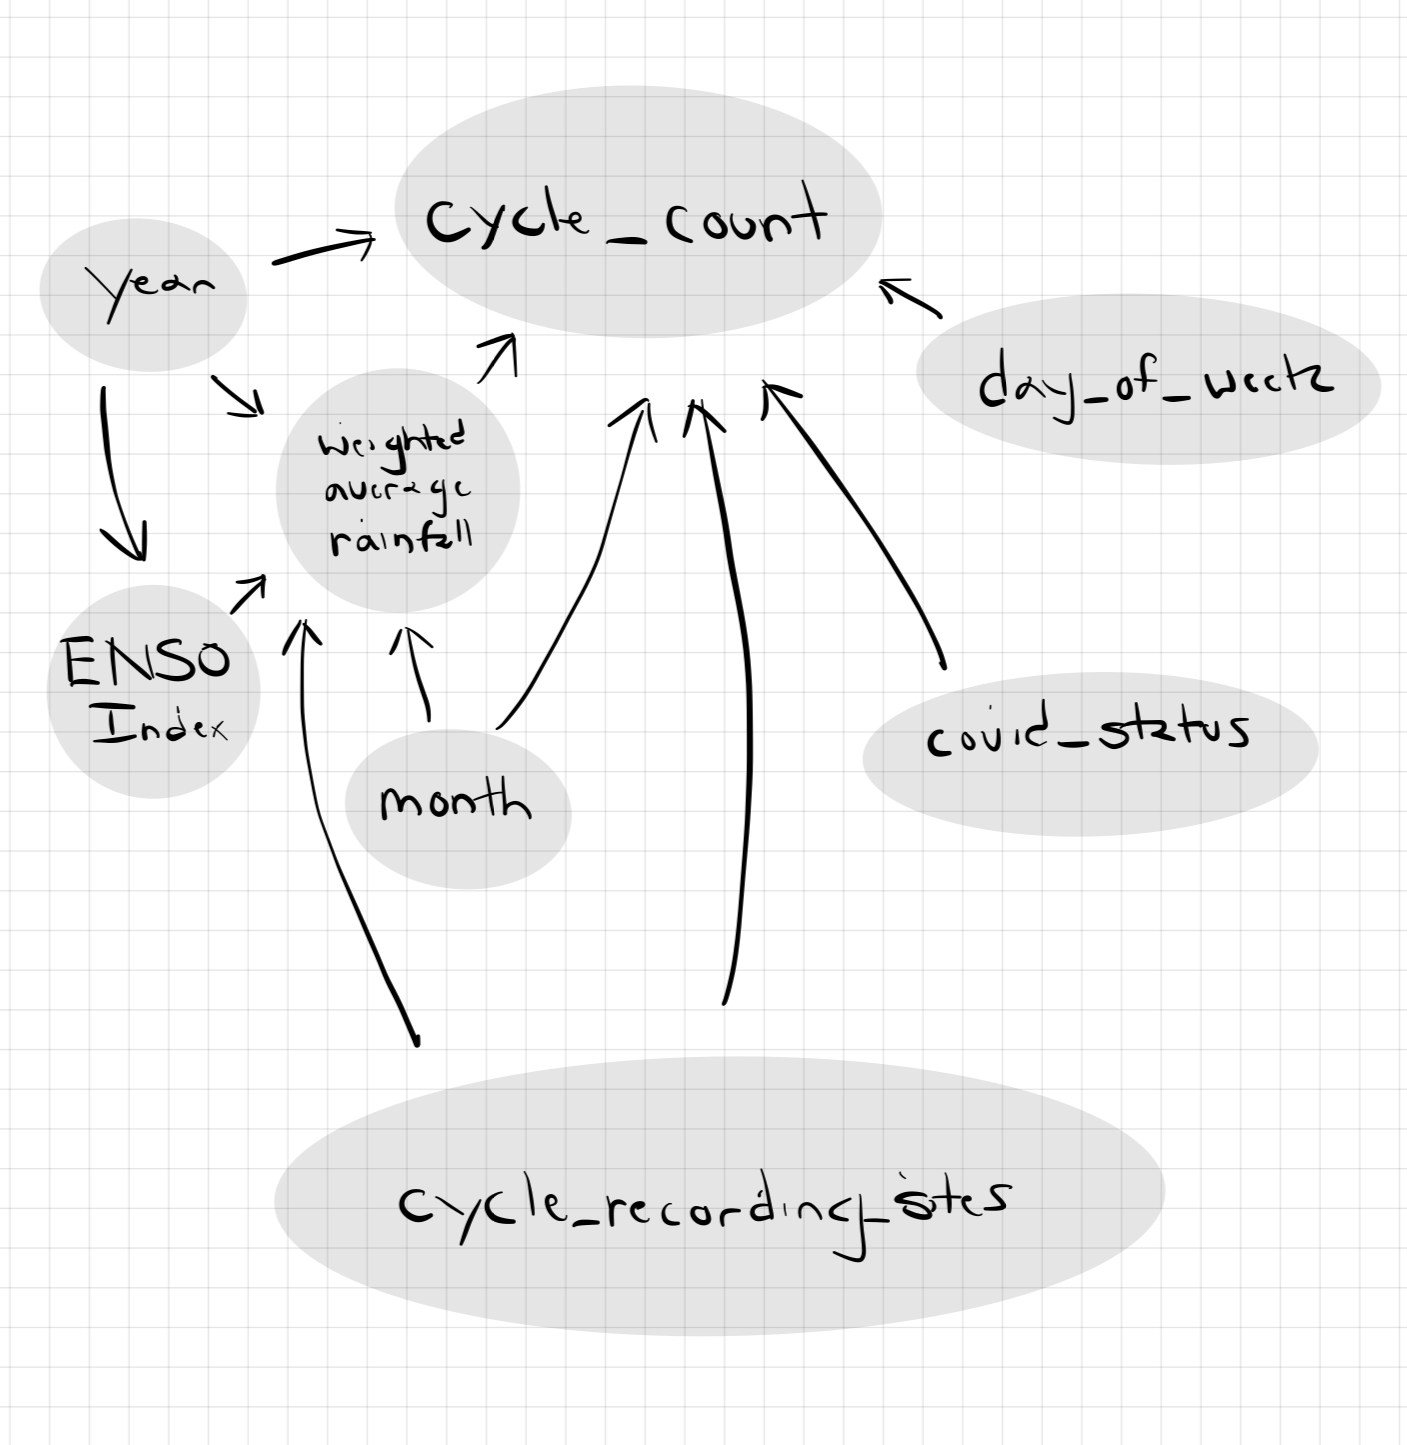
\includegraphics[width=19.54in]{data/cycle_count_causal_DAG}

I believe there aren't any relevant colliders or mediators for rainfall
on cycle count.

\hypertarget{bivariate-plots}{%
\paragraph{Bivariate Plots}\label{bivariate-plots}}

These plots show direct relationships between the concerning covariate
with direct effects on cycle\_count and confounders of rainfall,
supporting our causal diagram.

\includegraphics{cycling-in-the-rain_files/figure-latex/unnamed-chunk-11-1.pdf}

There was noticeably more cycle counts in 2019. There appears to be an
overall downward trend on cycling counts across the years. People often
cycle for leisure or transport (usually to and from work). Since
COVID-19, there has been a rise of hybrid/remote work, which in
combination with lockdowns, could explain the downward trend in cycle
counts. We include year in our model. We include year in our model as
this should have direct effects on cycle counts and a confounder of
rainfall on cycle counts.

\includegraphics{cycling-in-the-rain_files/figure-latex/unnamed-chunk-12-1.pdf}

There appears to be seasonality - the colder months (June, July, and
August) appear to have less cycle total counts compared to warmer months
(December, January, February, March). There are unusually low total
cycle counts in December, this could be due to the Christmas Holidays.
We include month in our model as this should have direct effects on
cycle counts and a confounder of rainfall on cycle counts.

It would be interesting to see the trend and seasonality across all
dates. Although dates will not be used in our model.

\includegraphics{cycling-in-the-rain_files/figure-latex/unnamed-chunk-13-1.pdf}

The plot of total cycle counts vs date supports the seasonality seen
between month and total cycle count, and downward trend seen between
year and total cycle count.

However these trends and seasonality are disrupted during the COVID-19
lockdowns, hence why we need to adjust for the COVID status covariate
when fitting our model.

\includegraphics{cycling-in-the-rain_files/figure-latex/unnamed-chunk-14-1.pdf}

There appears to be seasonality - the middle of the weekday (Tuesday and
Wednesday) has the highest total cycle counts, whereas the weekend
(Saturday and Sunday) have the lowest total cycle counts. This supports
the assumption that people often cycle for leisure or transport (usually
to and from work), the middle of the weekday being when people are most
likely working. We include day of week in our model as it has direct
effects on cycle count.

\includegraphics{cycling-in-the-rain_files/figure-latex/unnamed-chunk-15-1.pdf}

I averaged the cycle counts across all dates and locations within a
given COVID status, this is because each status has different periods.
Note that averages can be biased due to other seasonal and trend
effects.

There appears to be a higher average cycle count before the COVID-19
pandemic, which decreases significantly starting from the first lockdown
in March 2020. The ``post-COVID'' period also shows a noticeably lower
average cycle count. The primary focus of this analysis is to model the
relationship between rainfall and cycle counts. Although predicting and
explaining cyclist behavior during the COVID-19 period is challenging,
we adjust for COVID status in our model to reduce noise as it directly
impacts cycle counts. However, our primary attention is not on the
inference of the COVID status covariate itself but rather on
understanding the relationship between rainfall and cycle counts.

\includegraphics{cycling-in-the-rain_files/figure-latex/unnamed-chunk-16-1.pdf}

There is non-uniformity between total cycle count vs cycle recording
site. Certain cycle recording sites such as NW Cycleway Kingslandm, Quay
St.~Eco Display Classic, and Quay St.~Spark Arena have more cycle counts
across the dataset compared to other cycle recording sites such as
Matakana. There seems be an effect of rural and urbanised recording
sites on total cycle count, with urbanised sites being more popular. We
include cycle recording site in our model as it has direct effects on
cycle count.

\includegraphics{cycling-in-the-rain_files/figure-latex/unnamed-chunk-17-1.pdf}

There appears to be some seasonality of year on rainfall, this could be
due to El Niño-Southern Oscillation (ENSO). We include year in our model
as a confounder for rainfall on cycle count, and don't need to include
ENSO index as year covariate should cover the effects of ENSO.

Note: The bands are caused by taking rainfall measurements on the same
day but at different sites with similar amounts of weighted average
rainfall.

\includegraphics{cycling-in-the-rain_files/figure-latex/unnamed-chunk-18-1.pdf}

There appears to be seasonality of month on rainfall - winter months
(June, July, and August) having the highest rainfall compared to other
months. January, a Summer month, has the lowest rainfall compared to
other months. We include month in as a confounder for rainfall on cycle
count.

\includegraphics{cycling-in-the-rain_files/figure-latex/unnamed-chunk-19-1.pdf}

There is uniformity between rainfall vs cycle recording site. However
some sites (GI to Tamaki Dr.~Section 2, Matakana, New Lynn to Avondale
SUP, and Quay St.~Totem UZELT) appear to have much lower rainfalls than
all other sites, this is possibly due to the missing values in the data.

The uniformity could be due to not having local rainfall data which
accounts for micro-climates (i.e.~Matakana and Karangahape Rd. should
have different micro-climates). We are weighting the average between
measurements from only two rainfall stations based on distance, hence
why we would expect there to be less variation between rainfall across
all cycle recording sites.

Despite the limitation with our data, we still stand to include cycle
recording site in our causal diagram as a confounder for rainfall on
cycle count. Cycle recording site is still included in our model,
however it's estimates probably tell us more about the direct effects of
cycle recording site on cycle count.

\includegraphics{cycling-in-the-rain_files/figure-latex/unnamed-chunk-20-1.pdf}

\includegraphics{cycling-in-the-rain_files/figure-latex/unnamed-chunk-21-1.pdf}

A clear negative trend between rainfall and cycle count can be seen
across all sites and at each site. Higher rainfall measurements results
in less cycle counts, inversely lower rainfall measurements results in
more cycle counts.

There seems to be an inflated amount of 0 mm rainfall recordings.

\hypertarget{modelling}{%
\subsubsection{Modelling}\label{modelling}}

\hypertarget{poisson-model}{%
\paragraph{Poisson Model}\label{poisson-model}}

Since we are dealing with counts, we use a Poisson model as a first
step, with first order covariates and no interactions.

\begin{Shaded}
\begin{Highlighting}[]
\NormalTok{cycle\_count\_poisson\_model }\OtherTok{\textless{}{-}} \FunctionTok{glm}\NormalTok{(cycle\_count }\SpecialCharTok{\textasciitilde{}}\NormalTok{ weighted\_average\_rainfall }\SpecialCharTok{+}\NormalTok{ day\_of\_week }\SpecialCharTok{+}\NormalTok{ month }\SpecialCharTok{+}\NormalTok{ year }\SpecialCharTok{+}\NormalTok{ cycle\_recording\_site }\SpecialCharTok{+}\NormalTok{ covid\_status }\SpecialCharTok{{-}} \DecValTok{1}\NormalTok{, }\AttributeTok{family =} \FunctionTok{poisson}\NormalTok{(}\AttributeTok{link =} \StringTok{"log"}\NormalTok{), }\AttributeTok{data =}\NormalTok{ auckland\_cycle)}
\end{Highlighting}
\end{Shaded}

\begin{Shaded}
\begin{Highlighting}[]
\NormalTok{cycle\_count\_poisson\_model\_summary}
\end{Highlighting}
\end{Shaded}

\begin{verbatim}
## 
## Call:
## glm(formula = cycle_count ~ weighted_average_rainfall + day_of_week + 
##     month + year + cycle_recording_site + covid_status - 1, family = poisson(link = "log"), 
##     data = auckland_cycle)
## 
## Deviance Residuals: 
##     Min       1Q   Median       3Q      Max  
## -41.262   -4.572   -0.732    3.234  193.406  
## 
## Coefficients:
##                             Estimate Std. Error z value Pr(>|z|)    
## weighted_average_rainfall -2.525e-02  4.573e-05 -552.16   <2e-16 ***
## year2019                   4.189e-02  6.641e-04   63.08   <2e-16 ***
## year2020                   8.752e-02  1.049e-03   83.40   <2e-16 ***
## year2021                   1.051e-01  1.387e-03   75.77   <2e-16 ***
## year2022                   3.476e-01  8.077e-03   43.04   <2e-16 ***
## ---
## Signif. codes:  0 '***' 0.001 '**' 0.01 '*' 0.05 '.' 0.1 ' ' 1
## 
## (Dispersion parameter for poisson family taken to be 1)
## 
##     Null deviance: 239480046  on 79449  degrees of freedom
## Residual deviance:   4361284  on 79366  degrees of freedom
## AIC: 4907324
## 
## Number of Fisher Scoring iterations: 5
\end{verbatim}

The residual deviance appears a lot larger than the degrees of freedom,
this suggests over-dispersion. The next step would be to fit a negative
binomial model with a dispersion parameter.

The average effects of weighted average rainfall are: for every one-unit
(1 mm) increase of rainfall, the expected count of cyclists decreases by
a factor of \(e^{-0.02525} \approx 0.975\), or about \(2.5\%\) less.

\includegraphics{cycling-in-the-rain_files/figure-latex/unnamed-chunk-25-1.pdf}

\includegraphics{cycling-in-the-rain_files/figure-latex/unnamed-chunk-26-1.pdf}

The fit line looks quite noisy, however we can see that the line follows
the trend quite closely with cycle counts decreasing with increasing
rainfall measurement.

\includegraphics{cycling-in-the-rain_files/figure-latex/unnamed-chunk-27-1.pdf}

The variance of the scatter is not constant, it increases as the fitted
values increase, suggesting that there is over-dispersion. A solution is
use a negative binomial model.

\hypertarget{negative-binomial}{%
\paragraph{Negative Binomial}\label{negative-binomial}}

\begin{Shaded}
\begin{Highlighting}[]
\NormalTok{cycle\_count\_negbin\_model }\OtherTok{\textless{}{-}} \FunctionTok{glm.nb}\NormalTok{(cycle\_count }\SpecialCharTok{\textasciitilde{}}\NormalTok{ weighted\_average\_rainfall }\SpecialCharTok{+}\NormalTok{ day\_of\_week }\SpecialCharTok{+}\NormalTok{ month }\SpecialCharTok{+}\NormalTok{ year }\SpecialCharTok{+}\NormalTok{ cycle\_recording\_site }\SpecialCharTok{+}\NormalTok{ covid\_status }\SpecialCharTok{{-}} \DecValTok{1}\NormalTok{, }\AttributeTok{data =}\NormalTok{ auckland\_cycle)}
\end{Highlighting}
\end{Shaded}

\begin{Shaded}
\begin{Highlighting}[]
\NormalTok{cycle\_count\_negbin\_model\_summary}
\end{Highlighting}
\end{Shaded}

\begin{verbatim}
## 
## Call:
## glm.nb(formula = cycle_count ~ weighted_average_rainfall + day_of_week + 
##     month + year + cycle_recording_site + covid_status - 1, data = auckland_cycle, 
##     init.theta = 4.069766297, link = log)
## 
## Deviance Residuals: 
##     Min       1Q   Median       3Q      Max  
## -6.3553  -0.7794  -0.1173   0.4658  12.3624  
## 
## Coefficients:
##                             Estimate Std. Error z value Pr(>|z|)    
## weighted_average_rainfall -0.0209893  0.0002997 -70.031  < 2e-16 ***
## year2019                   0.0339994  0.0059227   5.740 9.44e-09 ***
## year2020                   0.1127775  0.0100965  11.170  < 2e-16 ***
## year2021                   0.1318295  0.0126806  10.396  < 2e-16 ***
## year2022                   0.2689079  0.0567426   4.739 2.15e-06 ***
## ---
## Signif. codes:  0 '***' 0.001 '**' 0.01 '*' 0.05 '.' 0.1 ' ' 1
## 
## (Dispersion parameter for Negative Binomial(4.0698) family taken to be 1)
## 
##     Null deviance: 72246831  on 79449  degrees of freedom
## Residual deviance:    83839  on 79366  degrees of freedom
## AIC: 926037
## 
## Number of Fisher Scoring iterations: 1
## 
## 
##               Theta:  4.0698 
##           Std. Err.:  0.0208 
## 
##  2 x log-likelihood:  -925868.5680
\end{verbatim}

The coefficient for weighted\_average\_rainfall has increased slightly.

The residual deviance appears a lot smaller now. The dispersion
parameter has been found to be 4.1.

The average effects of weighted average rainfall are: for every one-unit
(1 mm) increase of rainfall, the expected count of cyclists decreases by
a factor of \(e^{-0.0209893} \approx 0.979\), or about \(2.2\%\) less.

\includegraphics{cycling-in-the-rain_files/figure-latex/unnamed-chunk-31-1.pdf}

\includegraphics{cycling-in-the-rain_files/figure-latex/unnamed-chunk-32-1.pdf}

Fitted lines appear almost identical to the Poisson model, however
slightly less noise, and preserving the same trend where.

\includegraphics{cycling-in-the-rain_files/figure-latex/unnamed-chunk-33-1.pdf}

The residuals have less of a trend and appear much smaller for the
negative binomial model compared to the Poisson model. This is probably
the final model of choice.

\hypertarget{discussion}{%
\subsubsection{Discussion}\label{discussion}}

\hypertarget{interactions}{%
\paragraph{Interactions}\label{interactions}}

I did not include interactions, and used a first order model with all
the covariates of concern. An extension of this investigation would be
to explore interaction effects between certain covariates and their
effect on cycle count.

\hypertarget{zero-inflated-rainfall-measurements}{%
\paragraph{Zero-inflated Rainfall
Measurements}\label{zero-inflated-rainfall-measurements}}

There appears be zero-inflated rainfall measurements, although it would
be tempting to use a zero-inflated Poisson, that is only if the
dependent variable is zero-inflated. In this case we could fit a
compound Poisson model and account for over-dispersion like in our
negative binomial model of choice.

\hypertarget{seasonality}{%
\paragraph{Seasonality}\label{seasonality}}

Although I included the ENSO index in the causal diagram and is a
confounder for rainfall, I decided not to investigate this further in
the model, as I believe the El Nino / El Nina effects are already
explained by the year covariate.

\hypertarget{special-days}{%
\paragraph{Special Days}\label{special-days}}

Public holidays such as Easter, Christmas, and New Years to name a few,
are an important covariate which has direct effects on the cycle count.
This is a covariate I would model as an extension of this analysis, that
may serve to decrease noise, decreasing residual of rainfall on cycle
counts.

\hypertarget{other-weather-covariates-not-included-in-analysis}{%
\paragraph{Other Weather Covariates (Not Included in
Analysis)}\label{other-weather-covariates-not-included-in-analysis}}

Rainfall is a good indicator of weather conditions favorable for
cycling, however we should also consider temperate and wind speed in our
model, that may serve to decrease the residual of rainfall on cycle
counts. However I'm not well versed in climate science, and adjusting
for these other covariates might introduce mediator in our model which
could be a problem.

\hypertarget{weekend-effect}{%
\paragraph{Weekend Effect}\label{weekend-effect}}

Based on my research, it appears that rainfall effects are more
pronounced between weekdays and weekends in very large metropolitan
areas. I chose not to include this covariate in the Causal DAG and
model, as I suspect the weekend effect may be negligible in a smaller
city like Auckland. Additionally, our rainfall data is not the most
comprehensive, which might render this consideration less impactful.
Even if there were a slight effect, it should be adequately accounted
for by the day of week covariate.

\end{document}
